% ============================================================
%  Section 3 – Philosophical and Natural Foundations of UVIF
% ============================================================
\section{Philosophical and Natural Foundations of \uvif{}}
\label{sec:foundations}

\subsection{Variational Principles in Natural Systems}

The history of physics is populated by profound simplifications: the
realization that mechanics, optics, and electromagnetism can each be
derived from a \emph{single variational principle}---the principle of
least action, Fermat's principle of least time, Hamilton's principle.
In each case, the behavior of a physical system is not the outcome
of a push-pull causal chain but of the extremization of a functional
over all possible trajectories. The actual trajectory is the one that
makes the action stationary.

Variational principles are not just computational conveniences; they
reveal something deep about the structure of nature. They show that
seemingly complex dynamics are organized around an underlying
symmetry---a global constraint that shapes local behavior without
dictating it step by step. The Euler-Lagrange equations that arise
from variational calculus are the local expression of a global
coherence principle \citep{campos2021discrete}.

\uvif{} draws on this tradition. The Variational Equilibrium of an
intelligent system is its analog of a stationary action: not a
global minimum of a single cost, but a stable operating point of a
system of forces that collectively constrain the space of viable
intelligent behavior. The forces pull and resist in multiple
directions simultaneously; the equilibrium is the configuration
in which their combined effect can be sustained through time.

\subsection{Self-Organization and Dynamic Equilibrium in Nature}

Beyond physics, the natural world offers a second and equally deep
source of inspiration: \emph{self-organization}. Complex systems in
biology and ecology routinely generate ordered, functional structure
from the local interactions of components, without central control and
without an explicit design objective. Termite mounds, slime mold
networks, the vascular trees of leaves, the spatial patterns of
dryland vegetation---all are instances of self-organized structure
that arises from simple local rules and simple physical or chemical
gradients \citep{levin2005self,kefi2024selforg}.

What makes self-organized systems relevant to intelligence is that
their structure is \emph{adaptive}. The spatial patterns of dryland
vegetation do not simply appear; they shift in response to aridity
gradients, providing the ecosystem with a mechanism to buffer
increasing stress \citep{kefi2024selforg}. The patterns are not
optimized for any single function; they are organized around the
preservation of the system's capacity to function at all---its
\emph{viable region} in the space of environmental conditions.

This is exactly what \uvif{} formalizes. The Variational Equilibrium
manifold of an intelligent system is its viable region: the set of
states from which the system can maintain its core functions across
a range of perturbations. Self-organization is the spontaneous
process by which systems discover and inhabit this region without
explicit instruction.

\subsection{Homeostasis, Adaptation, and Long-Term Stability}

Physiology discovered the concept of homeostasis in the nineteenth and
early twentieth centuries through the work of Claude Bernard and Walter
Cannon \citep{billman2020homeostasis}. The core insight was that living
organisms maintain a stable internal environment---\emph{milieu
int{\'e}rieur}---despite the continuous flux of the external world.
This stability is not passivity; it is active, energetically costly
regulation through interlocking feedback mechanisms.

More recent work has refined this picture in two important directions.
First, \emph{adaptive homeostasis} shows that the regulatory setpoints
themselves shift transiently in response to sub-toxic signals, expanding
or contracting the homeostatic range to accommodate non-damaging
perturbations \citep{davies2016adaptive}. This is homeostasis with
a meta-level: not just maintaining a fixed state, but dynamically
adjusting what state is to be maintained.

Second, \emph{homeodynamics} recognizes that biological systems inhabit
not a single stable state but a landscape of multiple metastable states,
with organized transitions between them \citep{lloyd2001homeodynamics,
petitjean2025homeodynamics}. Health is not the occupation of one
fixed point but the capacity to navigate this landscape---to shift
between states when conditions demand it while remaining within the
viable region that supports life.

The implications for intelligence are clear. An intelligent system
that cannot shift its operating mode in response to changing conditions
is fragile. An intelligent system that can shift its operating mode
\emph{without losing coherence} is robust. The Variational Equilibrium
of \uvif{} captures the structured flexibility that homeodynamics
describes: it is a manifold, not a point---a region of viable operation,
not a fixed target \citep{giuliani2024stability,bich2025homeostasis}.

\subsection{Nature-Aligned Intelligence}

The phrase \emph{nature-aligned intelligence} in our title is
deliberate. It signals not a romantic attachment to the natural world,
but a methodological commitment: the conviction that the long-running
experiment of biological evolution has discovered principles of robust
adaptive organization that artificial intelligence has yet to fully
absorb.

Natural systems are not optimal by human-designed metrics. A forest
does not maximize timber yield. A cell does not maximize ATP production.
A brain does not maximize prediction accuracy on any single task. What
they do is \emph{maintain the conditions for their own continued
functioning} across a wide range of circumstances and timescales. This
is the kind of intelligence that \uvif{} aims to formalize: not the
intelligence of the Olympic sprinter, optimized for one event, but the
intelligence of the experienced traveler, who knows how to remain
functional across unknown terrain.

Nature-inspired computing has long drawn on evolutionary algorithms,
swarm intelligence, and neural architectures inspired by the brain
\citep{jiao2024natureinspired,dhamdar2024biomimicry}. \uvif{} goes
deeper: it does not borrow the mechanisms of nature but its
\emph{organizing principles}---variational balance, homeodynamic
stability, self-organized resilience.

\begin{figure}[!t]
\centering
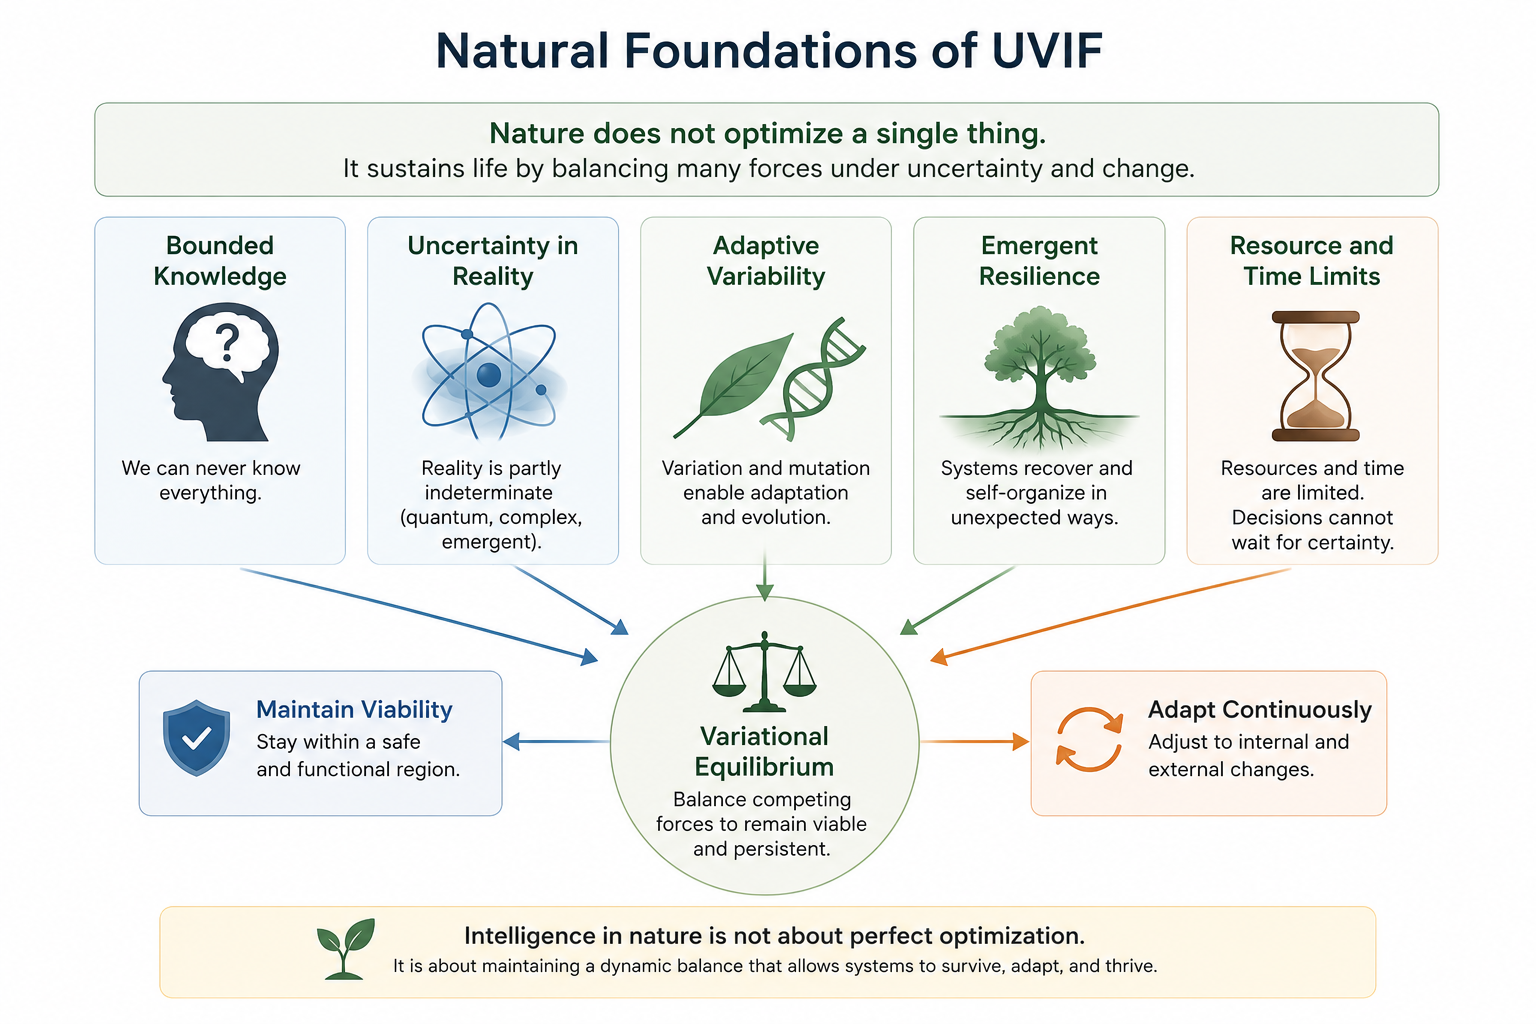
\includegraphics[width=\linewidth]{Figures/Fig3_Natural_Foundations.png}
\caption{Natural foundations of UVIF. Nature does not optimize a single
objective in isolation. Instead, biological and ecological systems
maintain viability through adaptive balance under uncertainty, resource
limitations, environmental variability, and incomplete knowledge. UVIF
adopts these organizational principles and interprets intelligence as
the maintenance of sustainable equilibrium rather than isolated
maximization.}
\label{fig:natural_foundations}
\end{figure}

Fig.~\ref{fig:natural_foundations} illustrates the central intuition
behind nature-aligned intelligence. The figure does not claim that
nature is consciously intelligent. Rather, it highlights that persistent
natural systems tend to survive through balance, adaptation, and
self-regulation rather than through aggressive optimization of a single
quantity.

The upper part of the figure summarizes several important observations
about natural systems. First, knowledge is always bounded: organisms and
systems never possess complete information about their environments.
Second, uncertainty is structurally embedded in reality itself, meaning
that adaptive systems must operate despite incomplete predictability.
Third, variability and mutation are not merely defects but mechanisms
that allow adaptation and long-term evolution. Finally, all natural
systems operate under limited resources and limited time, which means
that decisions cannot wait indefinitely for perfect certainty.

The center of the figure introduces the key concept of
\emph{Variational Equilibrium}. In the UVIF interpretation, intelligent
systems remain viable not by maximizing one variable, but by balancing
multiple competing pressures while continuously adapting to changing
conditions. The equilibrium region therefore represents a sustainable
operating zone rather than a single optimal point.

The lower part of the figure emphasizes the practical consequence of
this philosophy. Intelligence in nature is not about achieving perfect
optimization. It is about maintaining adaptive functionality across
changing environments and perturbations. UVIF adopts this principle as a
foundation for the design of resilient, sustainable, and uncertainty-aware
intelligent systems.


\subsection{From Control-Oriented Systems to Equilibrium-Oriented Systems}

Classical control theory provides a second lineage for \uvif{}. Control
systems maintain a desired system state by computing and applying
corrective actions. Proportional-integral-derivative (PID) controllers,
linear quadratic regulators, and model predictive control all operate
within this paradigm. They are powerful and well-understood within their
domain.

Yet control theory, as traditionally formulated, shares the
single-objective limitation of optimization. The controller is designed
to minimize a cost that reflects the deviation from a desired setpoint.
The setpoint is fixed by the designer. The system has no mechanism to
question whether the setpoint remains appropriate, or to balance the
cost of tracking the setpoint against other costs---energy expenditure,
actuator wear, safety margins, environmental impact.

\uvif{} shifts from the control metaphor to the \emph{equilibrium}
metaphor. Rather than asking how a system should be driven toward a
desired state, it asks what the natural resting configuration of a
system is when all its internal forces are in balance---and how the
system can be designed so that this natural configuration is also the
one that serves its purpose. This is the move from \emph{exogenously
imposed stability} (the controller drives the system to the setpoint)
to \emph{endogenously generated stability} (the system's internal
dynamics naturally converge to a viable operating region).

The free-energy principle in neuroscience makes a related move:
it describes perception and action as jointly minimizing a bound on
surprise, so that the system naturally comes to inhabit the sensory
states consistent with its generative model \citep{friston2010fep,
kim2022freeenergy}. \uvif{} extends and generalizes this insight
beyond the sensory-motor loop to encompass the full complexity of
intelligent organization across biological, artificial, and social
systems.



% =========================
% Added new philosophical subsections
% =========================

\subsection{Bounded Knowability and Irreducible Uncertainty}

The UVIF framework adopts the position that intelligent systems embedded within reality cannot attain complete simultaneous knowledge of all relevant variables governing their environment and future evolution. This condition of bounded knowability extends beyond engineering limitations and reflects deeper epistemological constraints associated with observation, interaction, temporal evolution, and uncertainty \citep{lieder2019resourcerational}.

Physical systems themselves illustrate this principle. Quantum uncertainty demonstrates that certain properties cannot be simultaneously specified with arbitrary precision. UVIF does not claim that all intelligent systems are quantum systems in a computational sense. Rather, the uncertainty principle serves as an illustration that reality may fundamentally constrain exhaustive simultaneous disclosure \citep{busch2007heisenberg,fankhauser2025epistemic}.

This insight carries profound implications for intelligence. If complete certainty is unattainable, then intelligence cannot be defined as the asymptotic elimination of uncertainty. Instead, intelligence becomes the capacity to sustain coherent and adaptive operation under structurally incomplete knowledge.

Natural systems continuously operate under this condition. Organisms regulate physiology without complete environmental predictability. Ecosystems adapt without deterministic foresight. Human decision-making routinely proceeds despite incomplete information and uncertain futures. Waiting indefinitely for maximal certainty may itself become maladaptive when action delay threatens viability \citep{schulkin2019allostasis,davies2016adaptive}.

\subsection{Adaptive Indeterminacy and the Role of Variability}

Natural systems frequently exhibit probabilistic, stochastic, and partially indeterminate dynamics. Variability is not merely noise to be eliminated; it often serves as a condition enabling adaptation, resilience, exploration, and long-term evolution \citep{folke2006resilience,levin2005self}.

Biological mutation provides a central example. Evolutionary adaptation depends on controlled variability and probabilistic genetic transformation. A perfectly rigid and completely deterministic biological system would possess limited adaptive flexibility under changing environmental conditions \citep{barrett2008adaptation,matic2019mutation}.

Similarly, ecological systems exhibit fluctuating adaptive responses rather than rigid deterministic trajectories. Complex biological recovery processes, including spontaneous recovery phenomena observed in medicine, further suggest that highly interconnected systems may reorganize through mechanisms that remain only partially predictable from localized mechanistic descriptions \citep{challis1990spontaneous,radha2021spontaneous}.

UVIF interprets these observations as evidence that persistent intelligent organization does not emerge through rigid deterministic optimization alone. Instead, sustainable intelligence may require adaptive regulation under partially indeterminate and evolving realities. Variability, uncertainty, and incomplete disclosure therefore become structural conditions of long-term resilience rather than merely obstacles to be eliminated.
